\documentclass[11pt,a4paper]{article}
\usepackage[margin=2.3cm]{geometry}
\usepackage[T1]{fontenc}
\usepackage{lmodern,amsmath,amssymb,booktabs,tabularx,graphicx,float,microtype}
\usepackage[font=small,labelfont=bf]{caption}
\usepackage[colorlinks=true,linkcolor=blue,citecolor=blue,urlcolor=blue]{hyperref}
\usepackage{natbib}
\usepackage{enumitem}
\setlist{nosep,leftmargin=*}
\setlength{\parindent}{0pt}
\setlength{\parskip}{5pt}
\setlength{\emergencystretch}{2em}
\renewcommand{\topfraction}{0.9}
\renewcommand{\bottomfraction}{0.8}
\renewcommand{\textfraction}{0.08}
\renewcommand{\floatpagefraction}{0.75}
\setcounter{totalnumber}{4}
\newcolumntype{Y}{>{\raggedright\arraybackslash}X}
\newcommand{\E}{\mathbb E}
\newcommand{\Prob}{\mathbb P}
\newcommand{\Normal}{\mathcal N}
\title{Forecasting Eurovision Results and Voting Patterns\\[4pt]\large Country history, song characteristics, and the incremental value of bookmaker odds}
\author{Nikita Nazarov \qquad Ivan Tanaev}
\date{November 2026}
\begin{document}
\maketitle
\begin{center}\small
Data, code, and results: \url{https://github.com/ivantanaevv/eurovision-forecasting}
\end{center}
\begin{abstract}
We forecast three Grand Final outcomes: a top-ten finish, an audience rank above the jury rank, and the winner of each country's televote. Bayesian ranking, probit, and categorical-choice models are evaluated by expanding-window backtests for 2021--2024 and a separate 2025 test. To measure the contribution of bookmakers, we refit each feature model without odds on the same observations. Adding odds reduces the development-period top-ten Brier score by about 49\% and national-winner log loss by 33--37\%. It provides almost no improvement for audience--jury differences, where country-specific historical frequencies perform best. Hierarchical pair effects improve national-winner forecasts when odds are included, but their additional value without odds is small. The 2025 national-winner results are metric-dependent: odds improve log loss in both feature models, while worsening M1's Brier score and top-choice accuracy. Archived odds have no verified measurement time, so these gains describe predictive association in the archived data; their real-time attainability remains unverified.
\end{abstract}

\section{Forecasting problem and motivation}
Eurovision combines shared assessments of an entry with persistent differences in national preferences. A country may perform well overall while receiving unusually strong support from particular voters. We ask whether these patterns, together with measurable song and performance characteristics, help predict the next final, and how much information bookmaker odds add.

The intended forecast is issued at 12:00 UTC on the day of the Grand Final, after the finalists and running order are known. Outcomes are resolved that evening. The horizon is therefore within-day, conditional on qualification. Our exercise reconstructs historical forecasts; none of the reported predictions was publicly issued before the corresponding contest.

\begin{table}[H]\centering\small
\caption{Targets, forecast objects, and evaluation units.}\label{tab:targets}
\begin{tabularx}{\linewidth}{lYYY}
\toprule
Task & Target & Forecast & Scoring unit\\\midrule
A: top ten & $Y_{it}=\mathbf1\{R_{it}\leq10\}$ & Marginal top-ten probabilities derived from a distribution over complete rankings & Entry, averaged within each final\\
B: audience vs jury & $Y_{it}=\mathbf1\{R^{T}_{it}<R^{J}_{it}\}$; ties count as zero & Probability of the binary event & Entry, averaged within each final\\
C: national winner & $W_{vt}=i$, the recipient of voter $v$'s 12 televote points & Categorical distribution over eligible finalists & One national vote, averaged within year\\\bottomrule
\end{tabularx}
\end{table}

The three tasks share data but answer different questions. In particular, a probability of winning the entire contest is neither a top-ten probability nor a probability of winning a particular national vote. We use the market's overall-winner assessment as a predictor and estimate a separate mapping for each target.

\subsection{Relationship to prior research}
At the project-design stage, the lecturer suggested \citet{blangiardo2014}. Their Bayesian hierarchical ordinal-logit model studies scores awarded by voter--performer pairs in finals from 1998--2012. Its structured pair effects incorporate shared borders, migration, and latent cultural clusters. The paper reports some evidence of positive voting affinity, without comparable evidence of systematic negative bias under its criteria, and explicitly cautions against a causal interpretation.

This work motivated our use of persistent directed pair effects and partial pooling, which is useful when individual pairs have short histories. Our Task C instead models the single winner of each national televote through a categorical likelihood. Our criterion is predictive loss in future contests. We use distance, borders and lagged support, but do not reproduce the paper's migration covariates or latent cultural clusters. The connection to their paper is the use of hierarchical structure for recurring national preferences.

\section{Data and information available at forecast time}
\subsection{Sources and coverage}
Final results, participants and national scores are assembled from EurovisionAPI and checked against published Eurovision results and independent tables. Song and language variables come from the published Eurovision Song Science data \citep{adamska2025}; geography comes from Natural Earth v5.1.2. Odds are obtained from the closed-event Eurovisionworld archive. Source URLs are listed in the references and source records are retained in the data pipeline.

\begin{table}[H]\centering\small
\caption{Available data and the samples used for the matched odds comparison. Cancelled 2020 is excluded throughout.}\label{tab:data}
\begin{tabular}{lrrl}
\toprule
Data block & Years & Rows/events & Unit\\\midrule
Full finalist data & 2008--2025 & 437 & Finalist--year\\
Matched Task A & 2015--2025 & 259 & Finalist--year\\
Tasks B and C history & 2016--2025 & 232 & Finalist--year\\
Task C candidate table & 2016--2025 & 8,770 & Voter--recipient--year\\
Task C likelihood & 2016--2025 & 349 & National voting events\\
Bookmaker quotes & 2015--2025 & 1,295 & Five prices for each of 259 finalists\\\bottomrule
\end{tabular}
\end{table}

Task C retains voting countries that did not qualify for the final. Self-voting is excluded. Rest of the World is excluded as a national voter, as are San Marino's substituted televotes in the nine relevant contests. These exclusions apply to complete choice sets and to the construction of pair histories. A zero score is a genuine observation; non-participation is not treated as zero support.

The pipeline checks complete final rosters, unique keys, exactly ten top-ten labels per final, and one winner per eligible national vote. National scores use the standard total of 58 points. The corrected 2019 results are used. The Netherlands' 2024 exclusion was announced before the chosen cutoff, so it is removed from that year's candidate set. Historical running slots and the resulting dense performance order are stored separately. In 2023 the host indicator refers to the United Kingdom.

The full finalist sample contains 46 countries across 17 contests, including 170 top-ten finishes. The split-ranking sample contains 43 countries; the audience places an entry above the jury in 114 of 232 observations (49.1\%). The units are country--year entries. Appendix~\ref{app:data} gives the annual sample sizes and numerical feature summaries.

\subsection{Predictors}
The common block has nine variables: normalized running position, host status, English-only and mixed-English indicators, tempo, danceability, dynamic complexity, log word count, and lyrical repetitiveness. Language without English is the reference category. The published numerical audio features are used as supplied; they were not independently re-extracted from every historical recording. Current YouTube popularity and detailed current-year semifinal results are excluded.

Two additional historical predictors are task-specific. Task A uses smoothed past final strength and its observation count. Task B uses the smoothed past audience--jury rank difference and its count. Task C uses past pair support and its count, together with log distance between capitals and a shared-land-border indicator. This gives 11, 11 and 13 predictors without odds, and 12, 12 and 14 with odds. Exact transformations appear in Appendix~\ref{app:features}.

History is calculated over the preceding five calendar years, without extending the window to replace 2020. Historical features always use years strictly before the forecast year. All continuous predictors are standardized using the training fold alone; binary indicators remain on their original scale. For C, song-level scaling uses unique recipient--year observations, avoiding repeated weighting of a song by the number of voting countries.

\subsection{What the collected data show}\label{sec:eda}
We use the descriptive analysis notebook to examine the candidate predictors before discussing the forecasts. The figures in this section summarize the full collected sample, including 2025. They describe associations in that sample; the fitted models and evaluation below still use the stated chronological splits.

\begin{figure}[!htbp]\centering
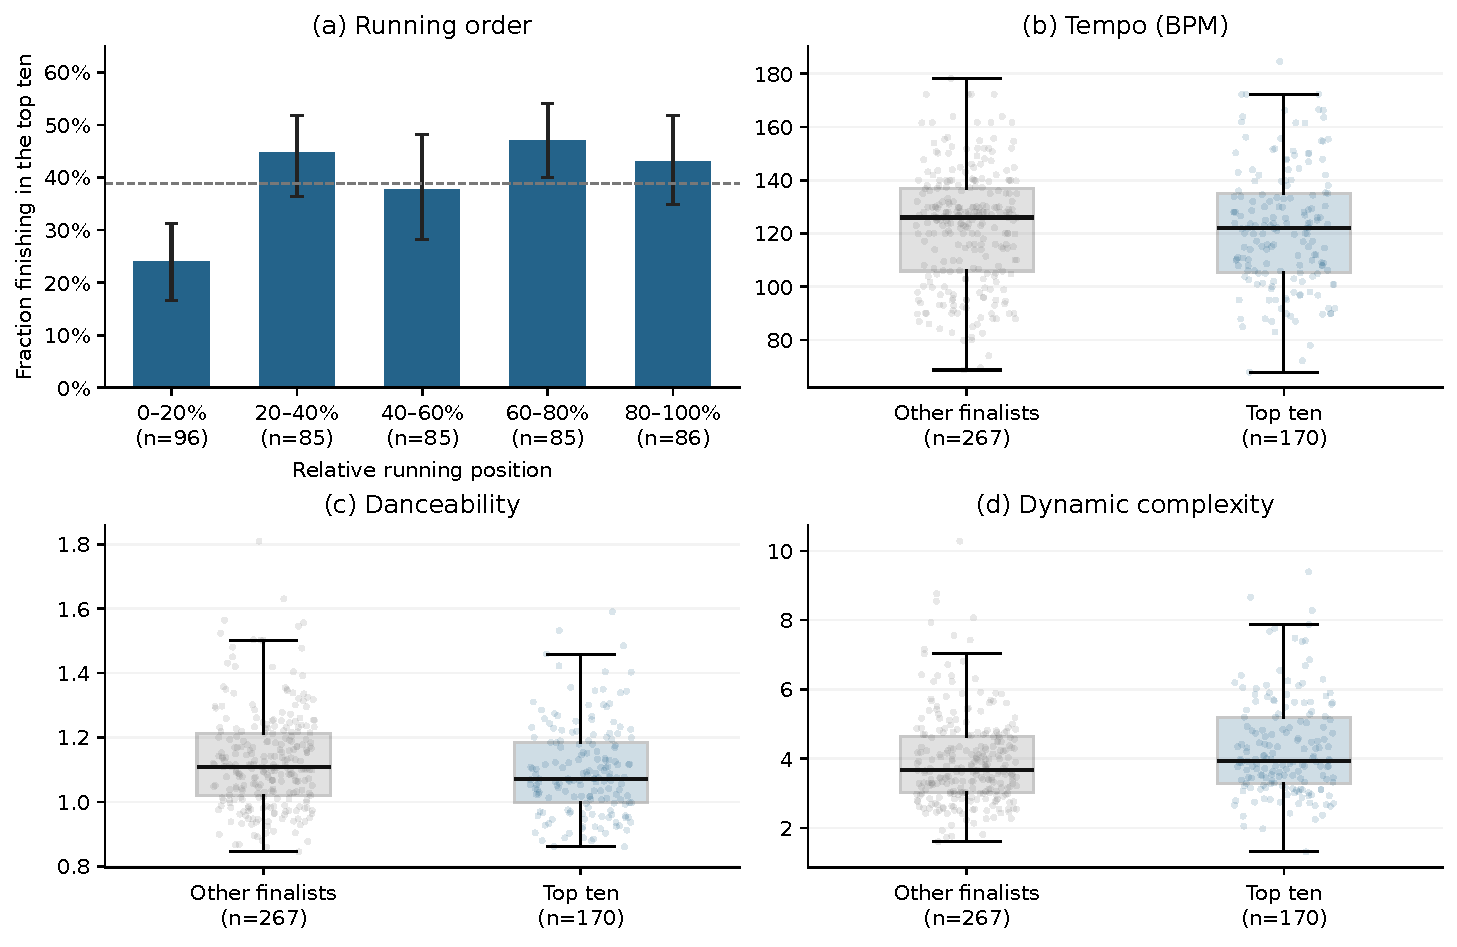
\includegraphics[width=\linewidth]{figures/data_song_patterns.pdf}
\caption{Running order and song characteristics, 437 finalists in 2008--2025. In (a), bars are pooled top-ten frequencies and intervals are 95\% bootstrap intervals from 3,000 resamples of whole years; the dashed line is the sample-average $10/N$. In (b)--(d), points show all observations, boxes show the interquartile range, and lines inside boxes show medians. Source: descriptive notebook, cells 3 and 6; rebuilt from the same processed data.}\label{fig:songdata}
\end{figure}

Only 24.0\% of entries in the first fifth of the running order reach the top ten, compared with 43.0\% in the last fifth. The pattern is not monotonic: the highest rate, 47.1\%, occurs in the 60--80\% group. Running position is therefore a plausible predictor, but these raw frequencies neither identify a causal advantage nor validate the linear specification used in our models.

The audio distributions overlap substantially. Median tempo is 121.9 BPM among top-ten entries and 126.0 among the others; their interquartile ranges are 105.3--134.9 and 105.9--137.1 BPM. Danceability and dynamic complexity also show broad overlap. This does not rule out joint predictive information, but it gives little support to a simple claim that faster or more danceable songs systematically succeed.

\begin{figure}[!htbp]\centering
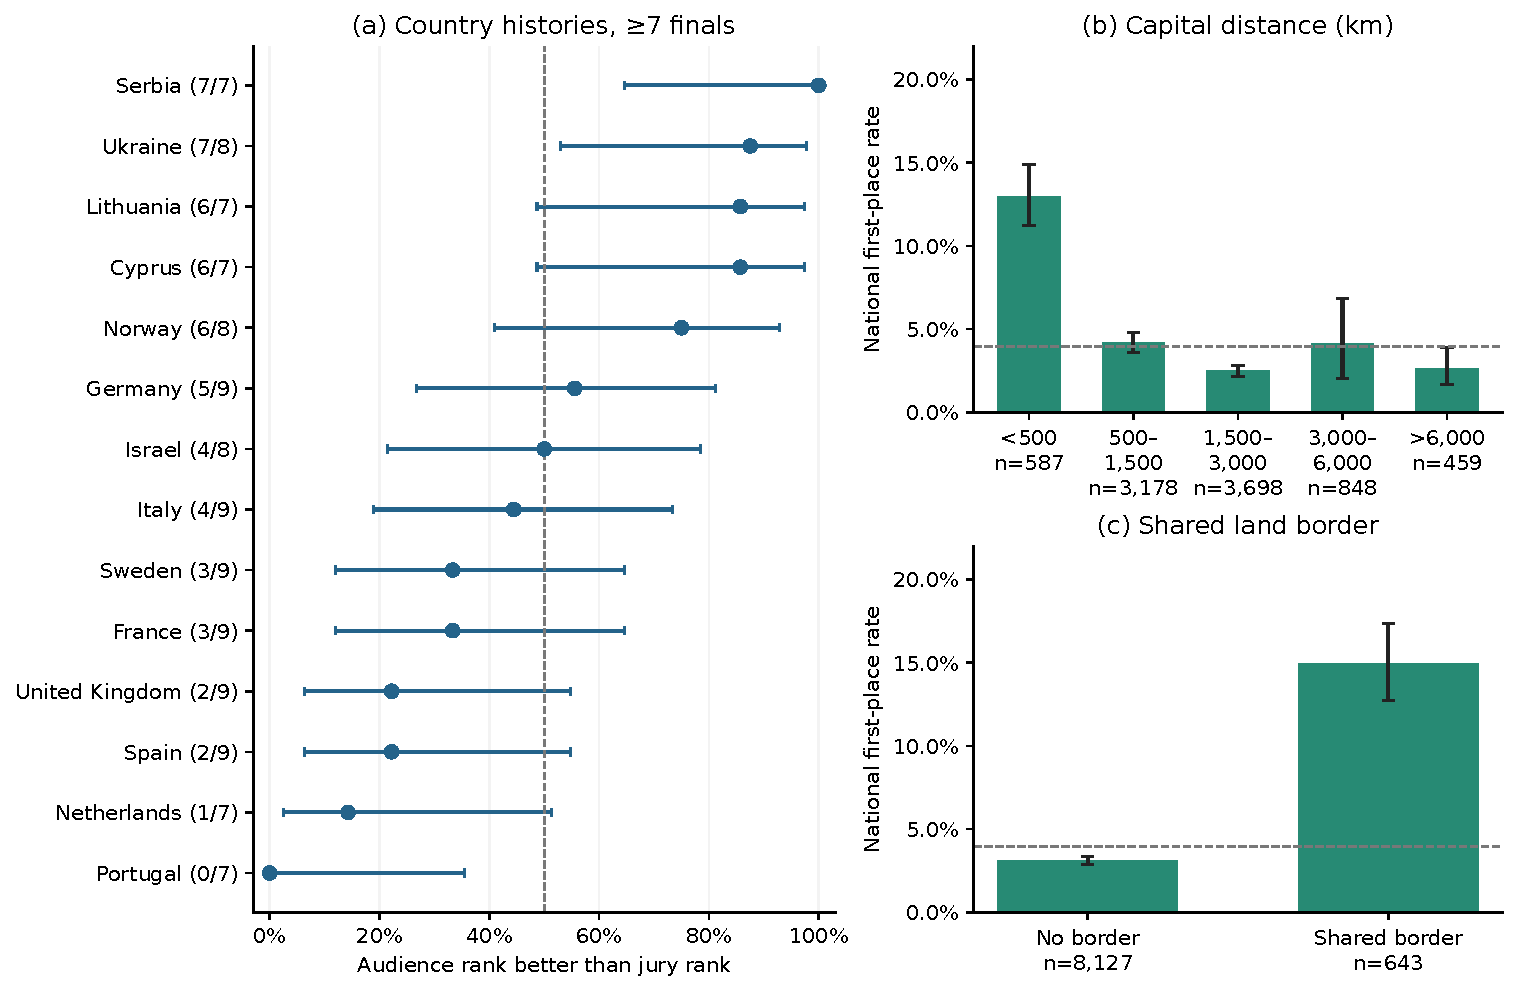
\includegraphics[width=\linewidth]{figures/data_country_geography.pdf}
\caption{Country histories and geography, 2016--2025. (a) Countries with at least seven finals; labels give successes/appearances and bars are approximate 95\% Wilson intervals. (b)--(c) National first-place frequencies among eligible voter--recipient pairs, with 95\% year-bootstrap intervals. The geographic dashed line is the row-average $1/K$, approximately 4\%. Candidate rows within a vote are mutually exclusive outcomes. Source: descriptive notebook, cells 4--5.}\label{fig:geodata}
\end{figure}

The country differences in B are large relative to the overall event frequency: Serbia places better with the audience than with the jury in all seven eligible finals, Ukraine in seven of eight, and Portugal in none of seven. Short histories make individual rates uncertain, as the intervals show. Country-specific probabilities with shrinkage are a reasonable baseline for this target.

In C, neighbouring countries award their national first place to one another in 14.9\% of eligible pair observations, compared with 3.1\% for pairs without a shared border. Pairs less than 500 km apart have a 12.9\% rate. These frequencies motivate distance, borders and pair history, but they also reflect which songs the countries sent and which years they participated. Appendix~\ref{app:pairs} compares selected bilateral frequencies with the recipient's support from other voters in the same years. Forecast evaluation is needed to determine whether these patterns help in a new contest.

\subsection{What the unknown odds timestamp means}\label{sec:timestamp}
The phrase in our presentation means that \emph{the time at which the archived prices were measured is not verified}. We retain the sources and retrieval records, but the date on which we retrieved an archive does not establish when its prices were originally quoted. Nor does a closed-event archive establish availability at 12:00 UTC, or the same number of hours before each final. We cannot rule out that some snapshots reflect information arriving after our intended cutoff.

All years use one source and the same five bookmakers: BET365, BETFRED, BoyleSports, SkyBet and Unibet. For finalist $i$, bookmaker $b$ and year $t$, we calculate
\begin{equation}
 q_{bit}=\frac{o_{bit}^{-1}}{\sum_{j\in F_t}o_{bjt}^{-1}},\qquad
 p^{\mathrm{mkt}}_{it}=\frac15\sum_{b=1}^{5}q_{bit},\qquad
 m_{it}=\log\!\left(\max\{p^{\mathrm{mkt}}_{it},10^{-6}\}\right).
\end{equation}
Here $F_t$ is the eligible finalist set and $o$ denotes decimal odds. Normalization is performed separately for each bookmaker before averaging. These are our normalized implied probabilities, not the site's rounded winning-chance column. 

We therefore report two experiments: a matched sample without odds and the same sample with archived odds. Their difference measures the incremental association of the archived market predictor with outcomes under the fitted models. A validated real-time forecasting gain would require timestamped quotes known to precede the cutoff. The no-odds experiment does not inherit this particular market-timing limitation.

\section{Models and estimation}
For each task we compare a historical baseline (M0), a model with predictors (M1), and a hierarchical extension (M2). All are probabilistic models; predictions average over posterior uncertainty. The baseline is deliberately informative: country history is available before the contest and provides a meaningful alternative to equal probabilities.

\subsection{Task A: a distribution over complete rankings}
Let $a_c$ be country $c$'s persistent strength and $x_{it}$ the predictors for entry $i$. The utilities are
\begin{equation}
 \eta_{it}^{(0)}=a_{c(i)},\qquad
 \eta_{it}^{(1)}=a_{c(i)}+x_{it}'\beta,\qquad
 \eta_{it}^{(2)}=a_{c(i)}+x_{it}'\beta.
\end{equation}
M0 and M1 use $a_c=0.5(z_c-\bar z)$ with independent $z_c\sim\Normal(0,1)$. M2 replaces the fixed scale by $\tau$, with $\tau\sim\mathrm{HalfNormal}(0.5)$. Thus M1 already has regularized country effects; M2 estimates their shared scale.

For observed complete ranking $\pi_t$, the Plackett--Luce likelihood is
\begin{equation}
 \Prob(\pi_t\mid\eta_t)=\prod_{k=1}^{N_t-1}
 \frac{\exp(\eta_{\pi_{tk},t})}{\sum_{j=k}^{N_t}\exp(\eta_{\pi_{tj},t})}.
\end{equation}
Each position is selected from the remaining participants. We simulate full rankings from each posterior draw and count top-ten appearances. Every simulated final has exactly ten such entries, so the marginal top-ten probabilities sum to ten. An overall intercept would cancel and is omitted. The model also supplies overall-winner probabilities, although top-ten prediction remains the primary target.

\subsection{Task B: audience rank above jury rank}
M0 assigns a separate probability to each country:
\begin{equation}
 \theta_c\sim\mathrm{Beta}(1,1),\qquad
 \widehat p_c=\frac{s_c+1}{n_c+2},
\end{equation}
where $s_c$ is the number of earlier successes and $n_c$ the number of earlier eligible finals. A country with no history receives probability $1/2$.

The feature models use $Y_{it}\sim\mathrm{Bernoulli}(\Phi(\eta_{it}))$. In M1,
$\eta_{it}=a_{c(i)}+x_{it}'\beta$ with independent $a_c\sim\Normal(0,1)$.
At zero predictors, $\Phi(a_c)$ has a uniform prior, consistent with M0's prior. M2 uses
\begin{equation}
 \eta_{it}=\alpha+x_{it}'\beta+\tau(z_{c(i)}-\bar z),\qquad
 \alpha\sim\Normal(0,1),\quad \tau\sim\mathrm{HalfNormal}(0.5).
\end{equation}
Predictions average $\Phi(\eta)$ across posterior draws. M1--M2 changes both the population-level structure and the treatment of the intercept. The product Bernoulli likelihood is an approximation for marginal events: it does not model the two full rankings jointly. Grouping forecast comparisons by year accounts for within-year dependence in evaluation, but does not remove this likelihood limitation.

\subsection{Task C: one winner per national vote}
For voter $v$ and finalist $i$, with admissible set $C_{vt}=F_t\setminus\{v\}$,
\begin{equation}
 \Prob(W_{vt}=i\mid\theta)=
 \frac{\exp(\eta_{vit})}{\sum_{j\in C_{vt}}\exp(\eta_{vjt})}.
\end{equation}
M0 uses $\eta_{vit}=a_i$, learning recipient strength from previous national winners. M1 adds song and pair predictors: $\eta_{vit}=a_i+x_{it}'\beta+w_{vit}'\gamma$. M0/M1 use the same fixed country-effect scale as Task A. M2 estimates that scale and adds a directed pair effect $d_{vi}$:
\begin{equation}
 \eta_{vit}=a_i+x_{it}'\beta+w_{vit}'\gamma+d_{vi},\qquad
 d_{vi}=\tau_d(Z_{vi}-\bar Z_{v\cdot}-\bar Z_{\cdot i}+\bar Z),
\end{equation}
where $Z_{vi}$ are independent standard normal variables and
$\tau_d\sim\mathrm{HalfNormal}(0.5)$. The full matrix is centered before ineligible candidates are masked. The effects $d_{vi}$ and $d_{iv}$ can differ. A voter-only intercept would cancel in the softmax and is omitted.

Each national vote contributes one categorical observation. Candidate rows are not independent binary trials. The forecast is the posterior mean softmax vector and sums to one. For C, M1--M2 measures the joint contribution of estimating hierarchical scales and adding residual pair effects; it cannot isolate these two changes. Geographic variables enter both feature models, so this comparison also does not isolate geography's incremental forecast value.

\subsection{Priors and computation}
Predictor coefficients have independent $\Normal(0,0.5^2)$ priors after training-fold standardization. The priors regularize a relatively small historical sample. Countries or pairs with no training observations are represented by their population prior.

The implementation uses NumPyro 0.19.0, JAX 0.7.2 and NUTS. The default is four chains, 1,000 warmup iterations and 1,000 retained draws per chain, with a longer retry when diagnostics fail. Task A simulates 25 rankings per retained draw. Task B's M0 is analytical. Checks cover likelihood normalization, masking, shift invariance, training-only scaling, and probability-sum constraints. Prior-predictive checks precede fitting, and prior scales are doubled in a separate 2024 sensitivity exercise. Diagnostics and sensitivity results are discussed in Section~\ref{sec:robustness}.

\section{Evaluation design}
\subsection{Matched expanding-window comparison}
For each test year $t\in\{2021,2022,2023,2024\}$, we train on all eligible observations with year less than $t$. Initial training begins in 2015 for A and in 2016 for B/C. For 2025, training ends in 2024. The 2025 outcomes are excluded from fitting and from the prior sensitivity exercise.

Both odds regimes read the same market-covered sheets of the workbook; the no-odds setting, \texttt{matched\_core}, removes only \texttt{market\_strength}. It does not add earlier years to A's training sample. This avoids attributing a change in training history to the market feature. The full 2008--2025 A dataset is documented for coverage but is not the sample underlying the comparisons in this report.

The no-odds runs were added after feedback on the presentation. They are a post-presentation diagnostic of the market's contribution. Although their fitting protocol excludes 2025 outcomes, the additional comparison was designed after the original 2025 results had been viewed. We retain 2025 as a separately reported test year, without describing this entire follow-up analysis as prospectively preregistered.

\subsection{Scores and uncertainty}
For binary targets A/B we use
\begin{equation}
 \mathrm{BS}_t=\frac{1}{N_t}\sum_i(p_{it}-y_{it})^2,\qquad
 \mathrm{LL}_t=-\frac{1}{N_t}\sum_i
 \{y_{it}\log p_{it}+(1-y_{it})\log(1-p_{it})\}.
\end{equation}
For C, one vote contributes $-\log p_{W_{vt}}$ and
$\sum_{i\in C_{vt}}(p_{vit}-\mathbf1\{W_{vt}=i\})^2$. The latter is the summed multiclass Brier score, without division by the number of candidates. Its magnitude is therefore not directly comparable to binary Brier scores. Lower values are better for all reported losses.

We first average within year, then equally across the four development years. C's supplementary accuracy is the fraction of national votes for which the highest-probability candidate wins. Logarithmic losses are computed from posterior-averaged probabilities, not by averaging conditional log losses. Task A additionally evaluates the complete ranking likelihood; this is distinct from the sum of marginal binary scores.

The notebooks report paired comparisons by resampling whole contest years. With only four development years, these intervals have very limited information about generalization to future contests. Overlapping training windows also induce dependence across forecast years. Year is the resampling unit, preserving within-contest dependence. The intervals are descriptive; the sample is too short for a reliable asymptotic significance test.

\section{Results}
\subsection{Top-ten forecasts: most of the improvement comes from odds}
\begin{table}[H]\centering\small
\caption{Task A: top-ten probability losses. M0 uses country history and has no odds predictor.}\label{tab:A}
\begin{tabular}{llrrrr}
\toprule
Model & Predictors & \multicolumn{2}{c}{2021--2024 mean} & \multicolumn{2}{c}{2025} \\ 
 & & Brier & Log loss & Brier & Log loss \\
\midrule
M0 & History only & 0.2266 & 0.6440 & 0.2036 & 0.5929 \\
M1 & Without odds & 0.2388 & 0.6751 & 0.2080 & 0.6059 \\
M1 & With odds & 0.1210 & 0.3891 & 0.1519 & 0.4439 \\
M2 & Without odds & 0.2382 & 0.6749 & 0.2055 & 0.6040 \\
M2 & With odds & 0.1218 & 0.3894 & 0.1519 & 0.4443 \\
\bottomrule
\end{tabular}

\end{table}
Without odds, adding song, performance and recent-history predictors does not improve on M0. M1's mean Brier rises from 0.2266 to 0.2388. Adding the market predictor reduces it to 0.1210, a reduction of approximately 49.3\% relative to the otherwise identical M1. Binary log loss moves in the same direction, from 0.6751 to 0.3891. M2 produces nearly the same results; estimating the country-effect scale adds little here.

The 2025 test supports the same ordering. M1's Brier falls from 0.2080 without odds to 0.1519 with odds, an improvement of 27.0\%. The gain is smaller than in the development period. As an illustration from the supplementary overall-winner output, M1 without odds ranks the eventual winner, Austria, 25th by winning probability (about 1.0\%). With odds, Austria is second (about 7.7\%), while Sweden is the favourite. The market predictor improves the ranking of the eventual winner without identifying it as the most likely outcome.

Country history cannot fully represent the quality of a new song. The large odds increment is consistent with markets aggregating information about that year's entry, reception or performance that our compact feature block misses. This is an interpretation of the pattern; unverified snapshot timing prevents us from attributing the entire gain to information available at the intended cutoff.

\begin{table}[H]\centering\small
\caption{Task A beyond top-ten membership: negative log posterior-predictive probability of the complete ranking and of the overall winner. Each final contributes one score. Lower is better. The last column is the probability assigned to Austria, the 2025 winner.}\label{tab:Aranking}
\begin{tabular}{llrrrrr}
\toprule
Model & Predictors & \multicolumn{2}{c}{Ranking log loss} & \multicolumn{2}{c}{Winner log loss} & $P(\mathrm{AT},2025)$ \\ 
 & & 2021--24 & 2025 & 2021--24 & 2025 & \\
\midrule
M0 & History & 58.046 & 59.694 & 2.950 & 3.657 & 0.0258 \\
M1 & No odds & 58.136 & 61.032 & 3.068 & 4.560 & 0.0105 \\
M1 & With odds & 46.972 & 57.480 & 0.947 & 2.564 & 0.0770 \\
M2 & No odds & 58.097 & 60.920 & 3.082 & 4.525 & 0.0108 \\
M2 & With odds & 47.194 & 57.467 & 0.949 & 2.569 & 0.0766 \\
\bottomrule
\end{tabular}

\end{table}
The market gain extends to the full ranking. M1's mean ranking log loss falls from 58.136 to 46.972 in development, and from 61.032 to 57.480 in 2025. However, the 2025 winner remains much less likely than the winners in the development contests: M1's winner log loss is 2.564 in 2025 versus a development mean of 0.947. A useful top-ten forecast can still assign a modest probability to the eventual overall winner.

\subsection{Audience versus jury: country history remains competitive}
\begin{table}[H]\centering\small
\caption{Task B: probability that the audience rank is better than the jury rank.}\label{tab:B}
\begin{tabular}{llrrrr}
\toprule
Model & Predictors & \multicolumn{2}{c}{2021--2024 mean} & \multicolumn{2}{c}{2025} \\ 
 & & Brier & Log loss & Brier & Log loss \\
\midrule
M0 & History only & 0.1955 & 0.5750 & 0.1598 & 0.4953 \\
M1 & Without odds & 0.2165 & 0.6227 & 0.1765 & 0.5275 \\
M1 & With odds & 0.2167 & 0.6237 & 0.1733 & 0.5208 \\
M2 & Without odds & 0.2202 & 0.6350 & 0.1752 & 0.5277 \\
M2 & With odds & 0.2208 & 0.6369 & 0.1733 & 0.5234 \\
\bottomrule
\end{tabular}

\end{table}
M0 has the lowest development Brier and log loss, and remains best in 2025. Odds barely change the feature-model forecasts: development Brier is 0.2165 without odds and 0.2167 with odds for M1. For M2 the corresponding values are 0.2202 and 0.2208. Such small changes do not support a useful market increment and may be sensitive to Monte Carlo variation and displayed rounding.

In 2025, odds improve M1's Brier from 0.1765 to 0.1733, but it still underperforms the baseline's 0.1598. Overall winning chances summarize combined contest strength; the event in B is a relative audience--jury preference. Strong entries may rank highly with both audiences, so an overall-winner market need not predict the sign of their rank difference. The results favour a simple country-specific history model for this particular target.

\subsection{National winners: geography and pair history help, with a larger market increment}
\begin{table}[H]\centering\small
\caption{Task C: losses for complete national-winner distributions. Brier is summed over candidates before averaging over votes.}\label{tab:C}
\begin{tabular}{llrrrr}
\toprule
Model & Predictors & \multicolumn{2}{c}{2021--2024 mean} & \multicolumn{2}{c}{2025} \\ 
 & & Brier & Log loss & Brier & Log loss \\
\midrule
M0 & History only & 0.9501 & 3.0670 & 0.9483 & 3.0618 \\
M1 & Without odds & 0.9137 & 2.7639 & 0.8001 & 2.2960 \\
M1 & With odds & 0.7296 & 1.8391 & 0.8272 & 2.1433 \\
M2 & Without odds & 0.9065 & 2.7588 & 0.8171 & 2.3578 \\
M2 & With odds & 0.6895 & 1.7457 & 0.8028 & 2.0749 \\
\bottomrule
\end{tabular}

\end{table}
Without odds, M1 improves mean log loss from 3.0670 to 2.7639 and raises average top-choice accuracy from 8.3\% to 24.2\%. M2 reduces log loss only slightly further, to 2.7588, with 26.8\% accuracy. Thus the non-market predictor block contains useful information about national choice on average, but an additional pair-effect hierarchy yields little improvement in log loss over these four years.

With odds, M1 reaches log loss 1.8391 and M2 reaches 1.7457. Relative to their no-odds versions, the reductions are 33.5\% and 36.7\%. Development top-choice accuracy rises to 41.3\% and 44.1\%, respectively. A common song-strength signal and voter-specific preferences appear complementary: once the market helps identify broadly competitive entries, the pair structure helps allocate national preferences among them.

The 2025 results qualify this conclusion. Adding odds improves M1 log loss from 2.2960 to 2.1433, but worsens its Brier from 0.8001 to 0.8272 and reduces correct top choices from 15 of 36 to 12 of 36. For M2, odds improve log loss from 2.3578 to 2.0749, Brier from 0.8171 to 0.8028, and correct top choices from 12 to 14. Among all tested C configurations in 2025, M2 with odds has the best log loss, while M1 without odds has the best Brier and accuracy. Log loss, squared probability error and winner selection capture different aspects of performance; a single ranking of the models would obscure this distinction.

\begin{table}[H]\centering\small
\caption{Task C selection accuracy. ``Top three'' means that the actual national winner is among the three highest-probability recipients. Development percentages are means of annual rates; 2025 entries are exact counts of national votes. These measures supplement the probability scores in Table~\ref{tab:C}.}\label{tab:Caccuracy}
\begin{tabular}{llrrrr}
\toprule
Model & Predictors & \multicolumn{2}{c}{2021--2024 mean} & \multicolumn{2}{c}{2025} \\ 
 & & Top one & Top three & Top one & Top three \\
\midrule
M0 & History & 8.3\% & 16.8\% & 3/36 & 16/36 \\
M1 & No odds & 24.2\% & 45.0\% & 15/36 & 22/36 \\
M1 & With odds & 41.3\% & 73.6\% & 12/36 & 21/36 \\
M2 & No odds & 26.8\% & 45.6\% & 12/36 & 23/36 \\
M2 & With odds & 44.1\% & 75.7\% & 14/36 & 24/36 \\
\bottomrule
\end{tabular}

\end{table}
The three-candidate coverage is also higher with odds in development: M2 increases from 45.6\% to 75.7\%. In 2025 the increase is only one national vote, from 23 to 24 of 36. The separate test year shows a much smaller improvement in candidate coverage.

\subsection{Direct answer: how much do bookmaker odds add?}
\begin{figure}[!htbp]\centering
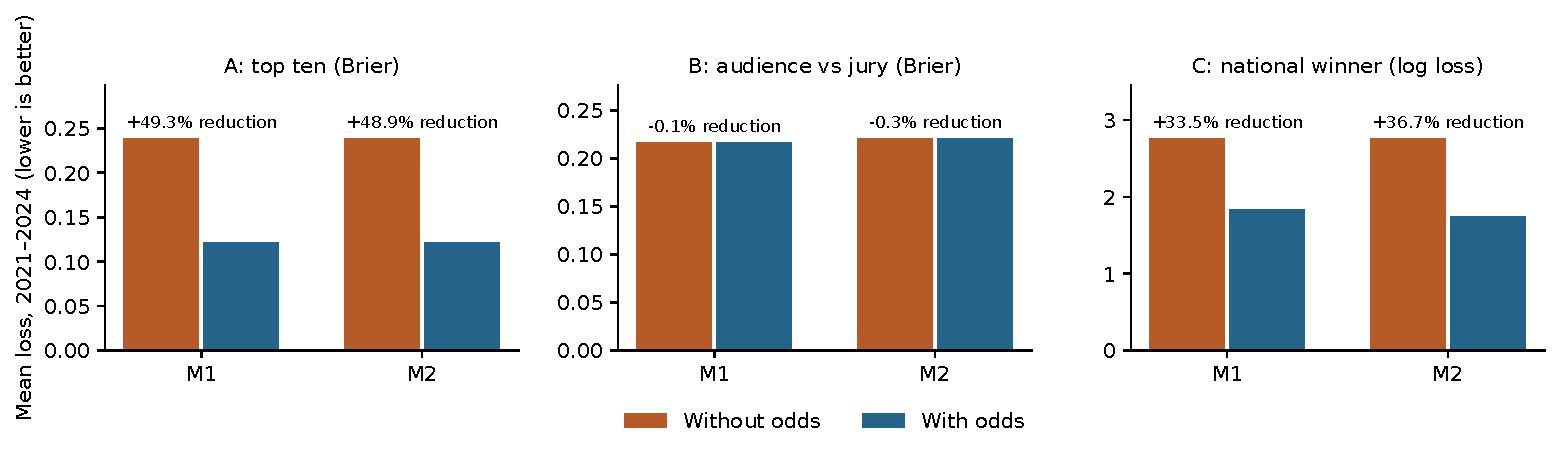
\includegraphics[width=\linewidth]{figures/market_increment.pdf}
\caption{Matched development-period comparison. Within each task and model, training years, test observations and non-market predictors are held fixed. Percentage labels give $(L_{\rm no\ odds}-L_{\rm odds})/L_{\rm no\ odds}$. The vertical scales differ by task.}\label{fig:increment}
\end{figure}
\begin{table}[H]\centering\small
\caption{Incremental market contribution. Positive numbers mean lower loss after adding odds. A/B use binary Brier; C uses categorical log loss.}\label{tab:increment}
\begin{tabular}{llrrrr}
\toprule
Task & Model & \multicolumn{2}{c}{2021--2024} & \multicolumn{2}{c}{2025} \\ 
 & & Loss reduction & Relative & Loss reduction & Relative \\
\midrule
A & M1 & +0.1178 & +49.3\% & +0.0561 & +27.0\% \\
A & M2 & +0.1164 & +48.9\% & +0.0536 & +26.1\% \\
B & M1 & -0.0002 & -0.1\% & +0.0032 & +1.8\% \\
B & M2 & -0.0006 & -0.3\% & +0.0019 & +1.1\% \\
C & M1 & +0.9248 & +33.5\% & +0.1527 & +6.7\% \\
C & M2 & +1.0131 & +36.7\% & +0.2829 & +12.0\% \\
\bottomrule
\end{tabular}

\end{table}
The largest increment is in A, a substantial increment appears in C, and almost none appears in B. These comparisons isolate adding one predictor within each specified architecture. They do not show that our feature models outperform a bookmaker-only model: such a benchmark was not fitted. They also do not identify the incremental value of song features or geography separately from the rest of the non-market block. Those questions require further matched ablations.

\begin{figure}[!htbp]\centering
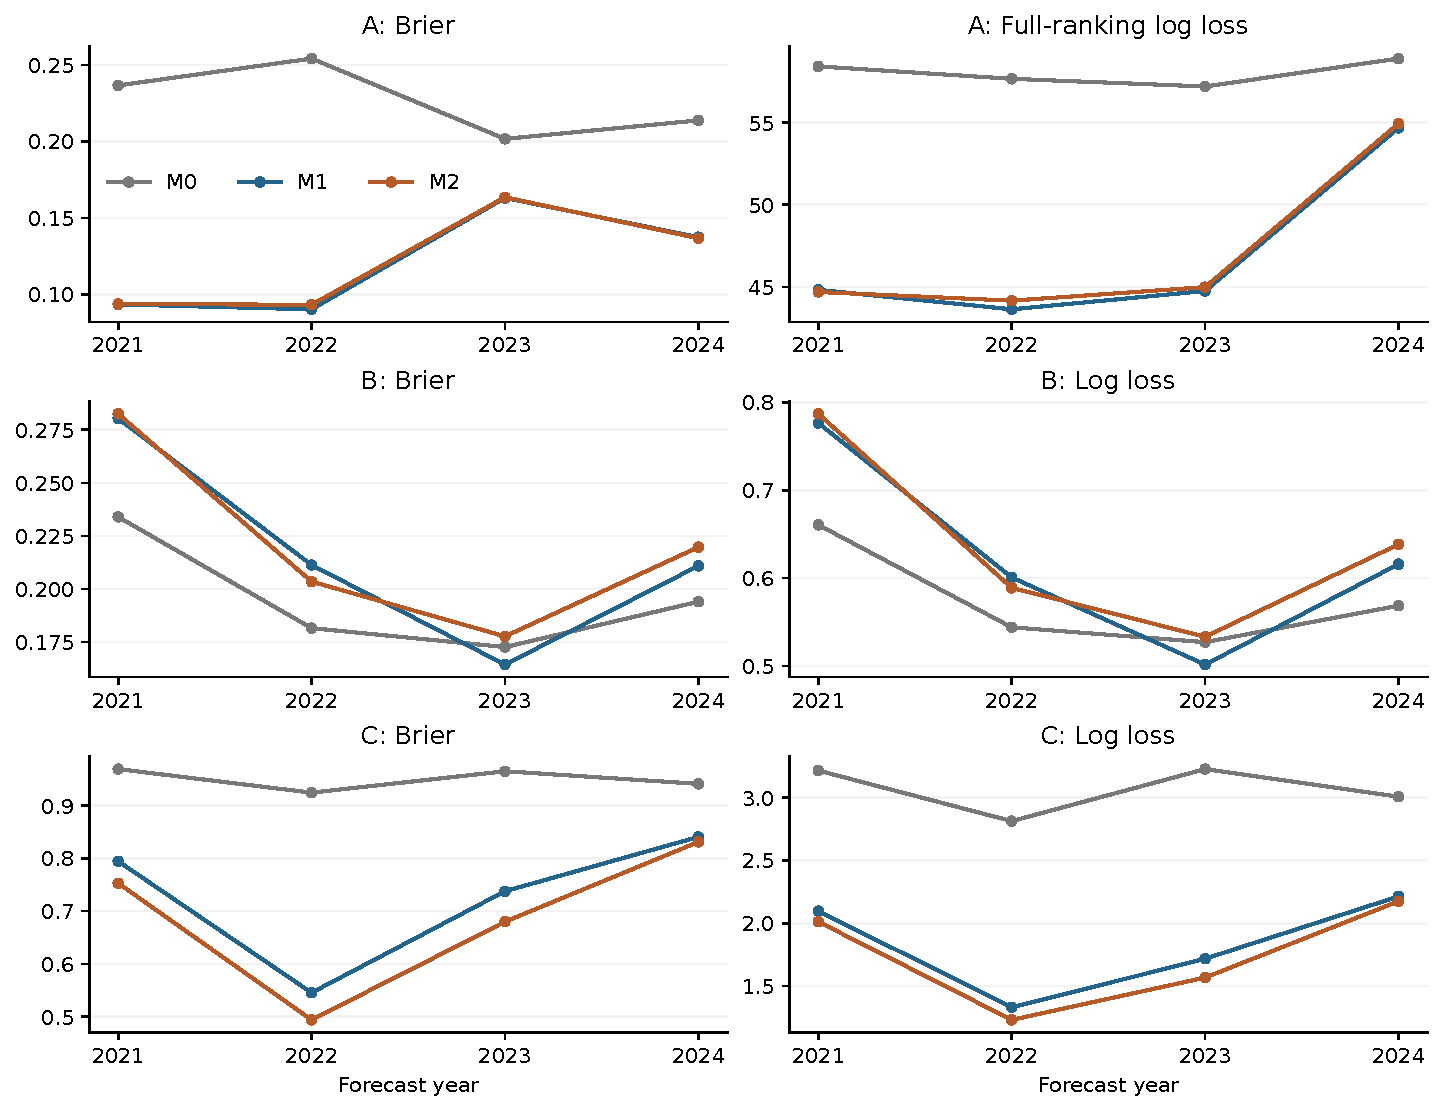
\includegraphics[width=\linewidth]{figures/annual_market_complete.pdf}
\caption{Annual development losses with odds, showing both scores plotted in the model notebooks. A's right panel scores the full ranking; its binary log loss is reported in Table~\ref{tab:A}. Each point uses a fresh fit on preceding years. The corresponding no-odds figures appear in Appendix~\ref{app:annual}.}\label{fig:annual}
\end{figure}
With odds, both feature models beat M0 on A and C losses in each development year. Their strongest C result is in 2022, while 2024 is substantially harder. In B, M0 is best in three of the four years; M1 wins in 2023. The no-odds plots reveal a further contrast: C's feature models deteriorate in 2024 and underperform M0 that year. Their mean gain without odds is therefore less stable than the aggregate table alone suggests.

\subsection{How the market changes individual forecasts}
\begin{figure}[!htbp]\centering
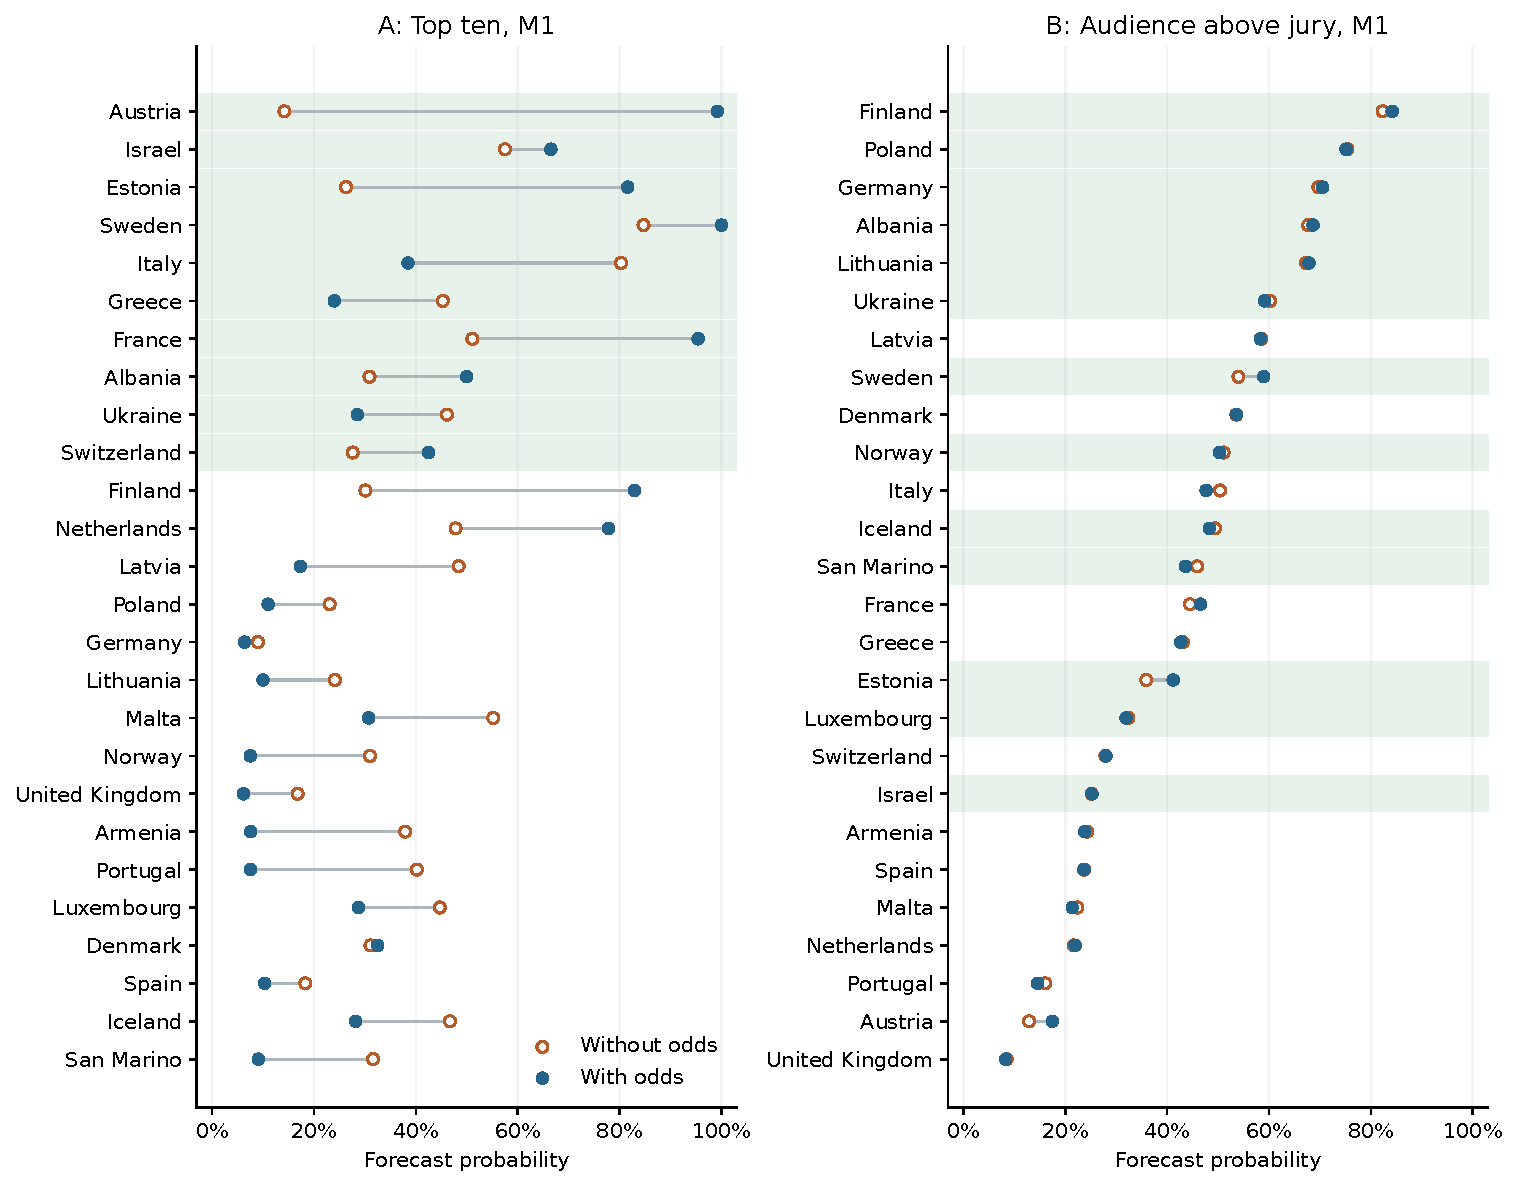
\includegraphics[width=\linewidth]{figures/forecast_ab_2025.pdf}
\caption{2025 M1 forecasts with and without odds. A row connects probabilities for the same country. Green shading marks a realized binary event. A is ordered by the actual final ranking; B by the no-odds probability. No-odds probabilities are extracted from notebook displays rounded to 0.1 percentage point.}\label{fig:ABforecast}
\end{figure}

In A, the market raises Austria's top-ten probability from 14.2\% to 99.2\% and Estonia's from 26.3\% to 81.6\%. It also raises Finland's to 82.9\% and the Netherlands' to 77.8\%, although both finish outside the top ten. Italy moves in the opposite direction, from 80.3\% to 38.4\%, despite finishing fifth. The aggregate improvement therefore contains both substantial corrections and new errors. In B, the two sets of probabilities are much closer, matching the small changes in the aggregate scores.

\begin{figure}[!htbp]\centering
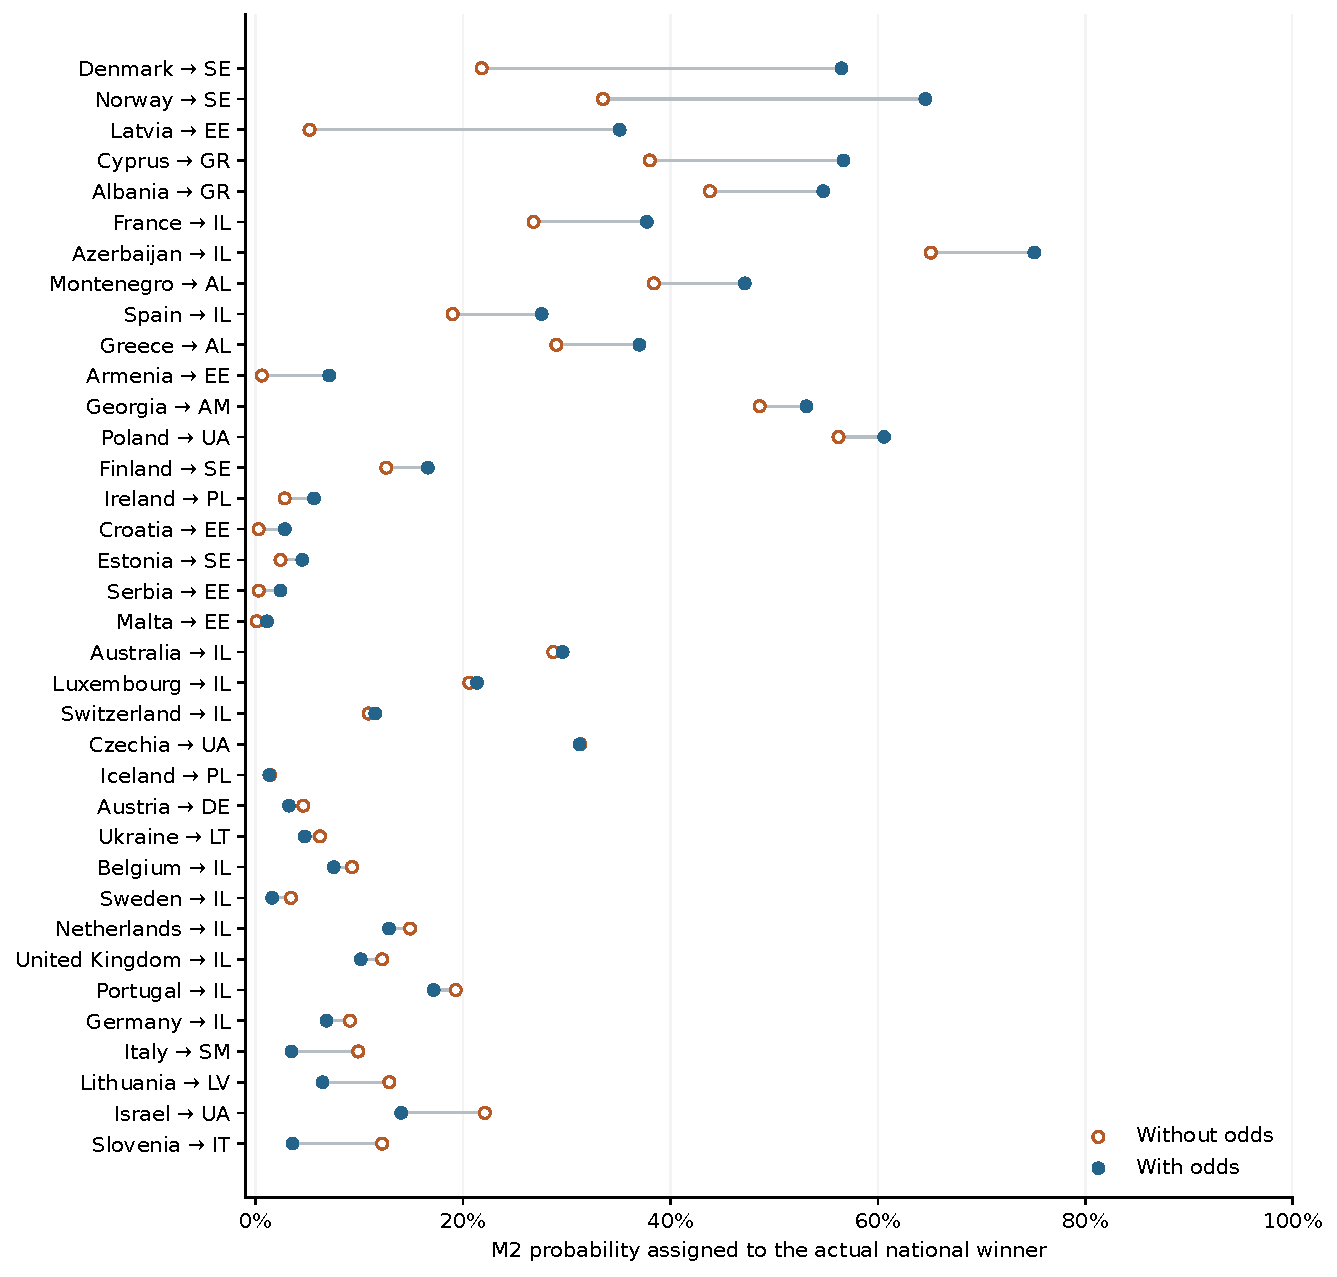
\includegraphics[width=.94\linewidth]{figures/forecast_c_2025.pdf}
\caption{Task C, 2025: M2 probability assigned to each observed national winner, with and without odds. Rows are ordered by the probability change. Recipient codes follow the dataset (for example, SE = Sweden and EE = Estonia). Each row is one of the 36 scoring events; this is a diagnostic of the realized outcomes. No-odds values retain notebook display precision.}\label{fig:Cforecast}
\end{figure}

The C log-loss gain is also uneven. For Denmark's vote for Sweden, M2's probability rises from 21.8\% to 56.5\%; for Latvia's vote for Estonia it rises from 5.2\% to 35.1\%. In contrast, the probability of Slovenia's eventual choice, Italy, falls from 12.2\% to 3.6\%. Because log loss directly penalizes the probability assigned to the actual winner, these changes help explain why odds improve the average without improving every national forecast.

\section{Interpretation, diagnostics and robustness}\label{sec:robustness}
\subsection{What the geographic and pair coefficients say}
\begin{figure}[!htbp]\centering
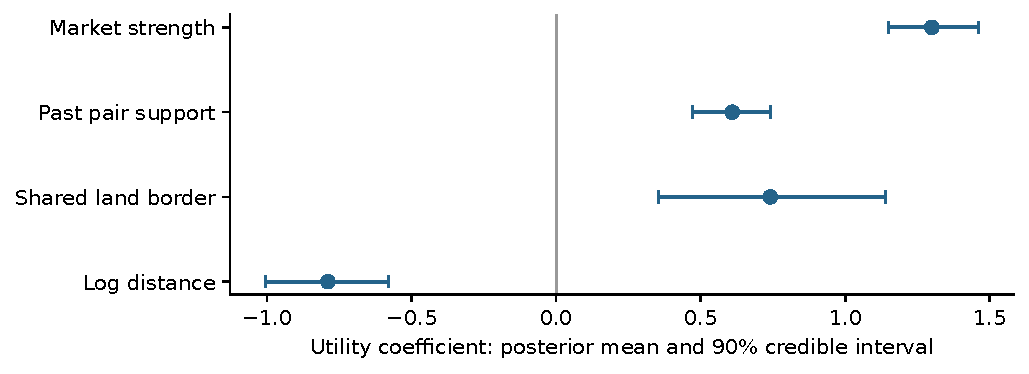
\includegraphics[width=.83\linewidth]{figures/pair_effects.pdf}
\caption{Selected Task C M2 coefficients with odds, fitted on years through 2024. Intervals are posterior 5th--95th percentiles. Continuous predictors are standardized; the border indicator is a change from zero to one. Coefficients are measured on the conditional utility scale.}\label{fig:effects}
\end{figure}
The estimated shared-border coefficient is 0.741 with a 90\% credible interval of $[0.355,1.139]$; the log-distance coefficient is $-0.789$ with interval $[-1.005,-0.579]$. Past pair support has a positive coefficient of 0.609, and market strength has a coefficient of 1.300. This pattern is consistent with both common entry strength and persistent bilateral preferences. It gives a concrete connection to the hierarchical motivation in \citet{blangiardo2014}, while leaving the mechanism of affinity unresolved. Geography may proxy language, migration, exposure or other omitted links. Moreover, model-based credible intervals condition on the assumed likelihood and do not establish out-of-sample gains from an individual variable.

\subsection{How strong is the evidence for hierarchy?}
\begin{table}[H]\centering\small
\caption{Task C paired development loss differences, M2 minus M1. Negative values favour M2. Intervals resample four whole years and should be read descriptively.}\label{tab:paired}
\begin{tabular}{llrrr}
\toprule
Predictors & Metric & Mean difference & 2.5\% & 97.5\%\\\midrule
Without odds & Log loss & $-0.0050$ & $-0.1218$ & $0.0991$\\
With odds & Log loss & $-0.0934$ & $-0.1339$ & $-0.0539$\\
Without odds & Brier & $-0.0073$ & $-0.0234$ & $0.0123$\\
With odds & Brier & $-0.0401$ & $-0.0546$ & $-0.0200$\\\bottomrule
\end{tabular}
\end{table}
For C with odds, the saved bootstrap intervals favour M2 on both scores. Without odds they include zero. For A without odds, the M2--M1 Brier difference is $-0.0006$, with interval $[-0.0028,0.0016]$; for B it is $0.0036$, with interval $[-0.0068,0.0122]$. The estimated scale extension has no clear advantage for A or B in these comparisons. In C the comparison also includes the new residual pair effects. Four years are too few to interpret the apparent separation in Table~\ref{tab:paired} as strong evidence of a stable future advantage.

For the market increment itself we report paired mean changes on matched samples. The supplied no-odds notebooks preserve rounded aggregate results and plots, but the per-year probability exports are unavailable in this package. A paired interval for the market increment cannot be recovered from the separate M1--M2 intervals and is not reported. A small change such as B's market increment should not be interpreted as statistically resolved.

\subsection{Computation and prior sensitivity}
Saved verification records for the market runs report maximum $\widehat R$ values of 1.0068 (A), 1.0067 (B) and 1.0082 (C), with zero divergences. Minimum bulk ESS values are approximately 631, 610 and 426, respectively. All three pass the implemented diagnostic gates. In the no-odds 2025 outputs, the largest $\widehat R$ is 1.0060, the smallest bulk ESS is about 664, and all fitted chains have zero divergences. C's no-odds M2 required a second, longer attempt. The checks address sampling accuracy; predictive adequacy is assessed by the backtests.

The 2024 no-odds sensitivity runs show that broader priors need not help. In A, doubling scales changes M1's Brier from 0.2309 to 0.2403; in B it changes M1's Brier from 0.2119 to 0.2254. In C, M1 log loss increases from 3.2971 to 3.5494 and M2 from 3.4354 to 3.6058. The 2025 forecasts use the original scales. These checks indicate that regularization is consequential in the small sample.

\begin{table}[H]\centering\small
\caption{Prior sensitivity of the no-odds feature models in the 2024 fold. Positive changes mean worse forecasts. A/B use Brier and C uses categorical log loss. This is a sensitivity exercise on one development year.}\label{tab:prior}
\begin{tabular}{lllrrr}
\toprule
Task & Model & Score & Original & Double scales & Change \\
\midrule
A & M1 & Brier & 0.2309 & 0.2403 & +0.0094 \\
A & M2 & Brier & 0.2276 & 0.2317 & +0.0041 \\
B & M1 & Brier & 0.2119 & 0.2254 & +0.0135 \\
B & M2 & Brier & 0.2218 & 0.2231 & +0.0013 \\
C & M1 & Log loss & 3.2971 & 3.5494 & +0.2523 \\
C & M2 & Log loss & 3.4354 & 3.6058 & +0.1704 \\
\bottomrule
\end{tabular}

\end{table}

\subsection{Calibration}
\begin{figure}[!htbp]\centering
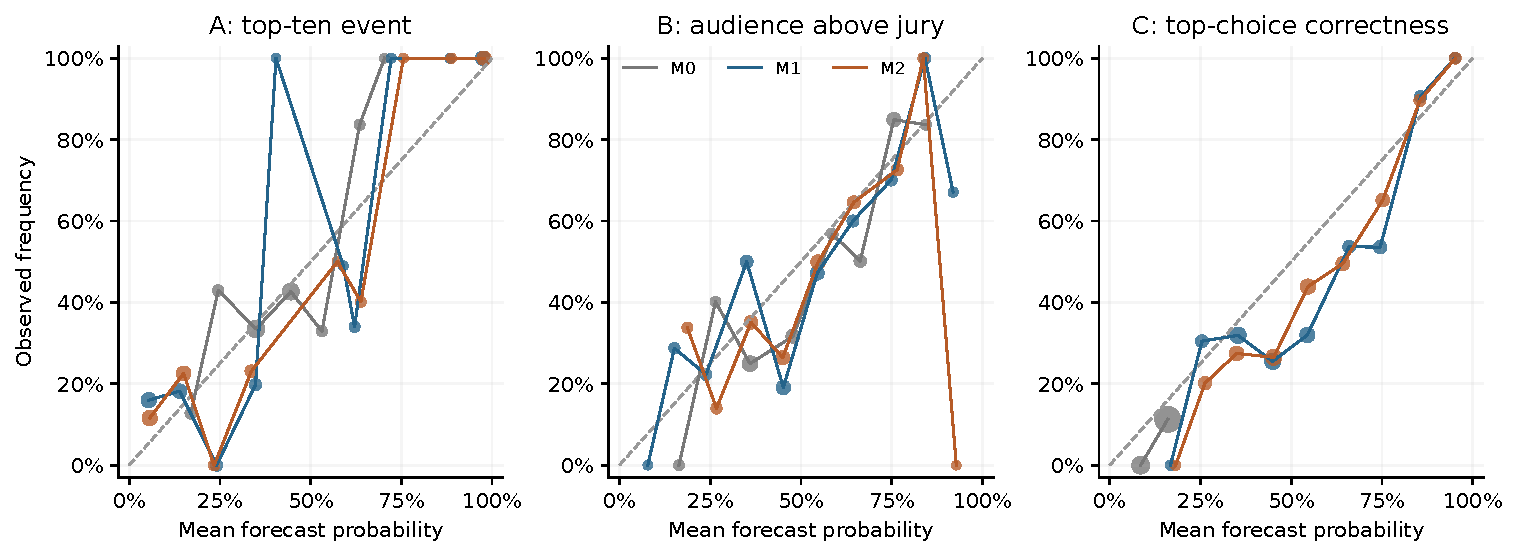
\includegraphics[width=\linewidth]{figures/calibration_market.pdf}
\caption{Development-period reliability diagrams for the market models. A/B calibrate binary event probabilities; C calibrates whether the highest-probability recipient wins. The diagonal represents calibration. Points use the saved year-weighted bin means; marker area increases with the number of observations in the bin. Lines join occupied bins and are not fitted calibration functions.}\label{fig:calibration}
\end{figure}
The curves show substantial departures from the diagonal in some bins, especially at extreme probabilities. Each A model has five occupied bins containing fewer than ten entries. With only four contests and dependent outcomes within each final, those bins cannot support precise calibration claims. The C diagram also answers a narrower question than calibration of the whole categorical vector: it checks confidence in the top choice. We use these plots to locate problems and retain Brier and log loss as the main quantitative comparisons.

\section{What the 2025 forecasts missed}
\begin{figure}[!htbp]\centering
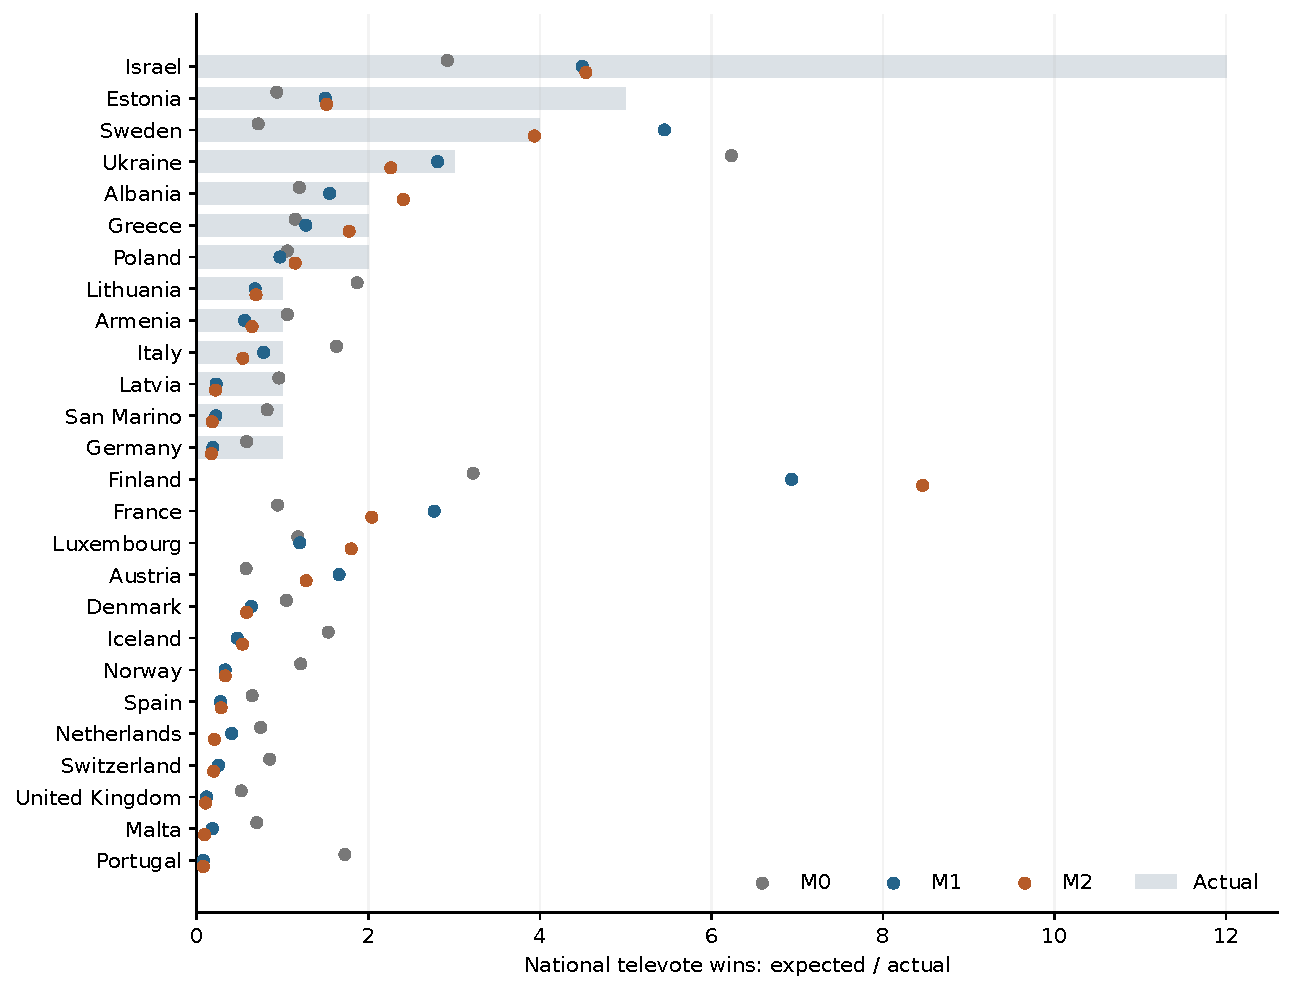
\includegraphics[width=.94\linewidth]{figures/national_win_counts.pdf}
\caption{Task C in 2025: observed national wins and sums of predicted probabilities, $\sum_v p_{vi}$, for the models with odds. Each series sums to 36. The forecast object is the number of national first places. The expectation requires no independence assumption across voters; a predictive interval for the count would require their joint distribution.}\label{fig:nationalcounts}
\end{figure}

The national-winner models miss part of the concentration of support in 2025. Israel receives 12 of the 36 national first places in our eligible sample, against 4.54 expected under M2 with odds. Estonia receives five, against 1.51 expected. Sweden is predicted much more accurately in this aggregate: 3.94 expected and four observed. M0's country history instead allocates 6.23 expected wins to Ukraine, which receives three. These discrepancies show where a stable country effect, a shared market predictor and bilateral adjustments remain insufficient.

The common year-specific component is a natural place to investigate. A broadly unexpected entry can receive support from many voters simultaneously, whereas our categorical likelihood treats national outcomes as independent conditional on the model parameters. The fitted hierarchy captures recurring pairs, but it has no additional contest-level shock shared by all national voters. The missed concentration is consistent with this explanation, although the experiment does not identify its cause. A useful extension would evaluate the distribution of national-win counts as well as the individual national probabilities.

For A, the missed top-ten forecasts for Finland and the Netherlands show that a strong market signal can also produce confident errors. For B, the country baseline remains difficult to improve on. Those findings set distinct priorities: richer current-entry information for A/C, and features that specifically distinguish audience from jury preferences for B. Adding the same popularity variable to every target is not enough.

Any further market experiment first needs quotes with verified pre-cutoff timestamps. A bookmaker-only model would then test whether the song and pair features add value beyond those quotes. Separate matched ablations could evaluate audio, language and geography. The present results establish the contribution of the full non-market block and the archived-odds increment; they do not identify each feature block's contribution. Changes in the final implementation relative to the proposal are documented in Appendix~\ref{app:proposal}.

\section{Conclusion}
For overall top-ten outcomes, the compact country/song feature models gain most of their predictive accuracy from the archived bookmaker predictor. For audience--jury differences, country-specific historical frequencies outperform the richer probit models, and the overall-winner market contributes little. National televote winners benefit from non-market pair and entry information, with a substantially larger development-period gain after odds are added. The hierarchical pair extension performs best by log loss with odds, but the 2025 results demonstrate that log loss, Brier and winner-picking accuracy need not select the same model.

The matched comparison gives a clear answer about this dataset: the market increment is large for A, substantial but less consistent across metrics for C, and negligible for B. Whether the same improvements can be obtained by a forecast issued at noon remains unresolved until the odds timestamps are verified.

\appendix
\section{Feature construction}\label{app:features}
Let $H_t=\{t-5,\ldots,t-1\}$, omitting 2020, and let $n$ count eligible observations in that window. The fixed smoothing strength is three neutral observations. For a country in A,
\[
 q_{cs}=\frac{N_s-R_{cs}}{N_s-1},\quad
 \mathrm{past\_final\_strength}_{ct}=\frac{\sum_{s\in H_t}q_{cs}+1.5}{n+3},\quad
 \mathrm{past\_final\_count}_{ct}=\log(1+n).
\]
For B, using comparable split results from 2016 onward,
\[
 \mathrm{past\_audience\_advantage}_{ct}
 =\frac{\sum_{s\in H_t}(R^J_{cs}-R^T_{cs})/(N_s-1)}{n+3},\qquad
 \mathrm{past\_split\_count}_{ct}=\log(1+n).
\]
For directed pair $(v,i)$ in C,
\[
 \mathrm{past\_pair\_support}_{vit}
 =\frac{\sum_{s\in H_t}(\mathrm{points}_{vis}-58/K_{vs})}{n+3},\qquad
 \mathrm{past\_pair\_count}_{vit}=\log(1+n),
\]
where $K_{vs}$ is the number of admissible candidates in that historical vote. Only real votes in which the recipient was eligible contribute. The neutral expected score is $58/K_{vs}$. Prior results from 2003--2007 support the earliest A features but are not included as rankings in the fitted likelihoods.

Running position is $(\mathrm{order}-1)/(N_t-1)$; word count enters as $\log(1+\mathrm{words})$. Geographic distance is the great-circle distance between mapped capitals, transformed as $\log(1+\mathrm{distance\ in\ km})$. Shared borders follow the fixed Natural Earth administrative coding; separately coded dependencies are not merged into their parent countries.

\section{Descriptive data tables}\label{app:data}
\begin{table}[H]\centering\small
\caption{Annual coverage. ``Audience $>$ jury'' counts a better audience rank. ``Votes'' counts eligible national choice events; ``candidate rows'' counts alternatives within those events. Zero split-ranking or market observations in the early years indicate unavailable coverage. There was no contest in 2020.}\label{tab:annualdata}
\begin{tabular}{rrrrrrr}
\toprule
Year & Finalists & Split ranks & Audience $>$ jury & Votes & Candidate rows & Odds \\
\midrule
2008 & 25 & 0 & 0 & 0 & 0 & 0 \\
2009 & 25 & 0 & 0 & 0 & 0 & 0 \\
2010 & 25 & 0 & 0 & 0 & 0 & 0 \\
2011 & 25 & 0 & 0 & 0 & 0 & 0 \\
2012 & 26 & 0 & 0 & 0 & 0 & 0 \\
2013 & 26 & 0 & 0 & 0 & 0 & 0 \\
2014 & 26 & 0 & 0 & 0 & 0 & 0 \\
2015 & 27 & 0 & 0 & 0 & 0 & 27 \\
2016 & 26 & 26 & 14 & 41 & 1040 & 26 \\
2017 & 26 & 26 & 15 & 41 & 1040 & 26 \\
2018 & 26 & 26 & 13 & 42 & 1066 & 26 \\
2019 & 26 & 26 & 12 & 40 & 1015 & 26 \\
2021 & 26 & 26 & 12 & 38 & 963 & 26 \\
2022 & 25 & 25 & 12 & 39 & 950 & 25 \\
2023 & 26 & 26 & 12 & 36 & 910 & 26 \\
2024 & 25 & 25 & 11 & 36 & 875 & 25 \\
2025 & 26 & 26 & 13 & 36 & 911 & 26 \\
\bottomrule
\end{tabular}

\end{table}

\begin{table}[H]\centering\small
\caption{Continuous entry features in the full 437-entry A dataset, before fold standardization. The two audio indices use the source dataset's scale; they are not restricted to $[0,1]$. Missing counts refer to the assembled modelling table.}\label{tab:datastats}
\begin{tabular}{lrrrrrr}
\toprule
Variable & Mean & SD & Q25 & Median & Q75 & Missing \\
\midrule
Running position & 0.50 & 0.30 & 0.24 & 0.50 & 0.76 & 0 \\
Tempo (BPM) & 122.22 & 21.94 & 105.81 & 123.86 & 136.03 & 0 \\
Danceability & 1.12 & 0.15 & 1.01 & 1.10 & 1.20 & 0 \\
Dynamic complexity & 4.08 & 1.36 & 3.12 & 3.79 & 4.76 & 0 \\
Log word count & 5.43 & 0.34 & 5.25 & 5.48 & 5.67 & 0 \\
Repetitiveness & 0.50 & 0.16 & 0.39 & 0.51 & 0.62 & 0 \\
\bottomrule
\end{tabular}

\end{table}

\begin{table}[H]\centering\small
\caption{Twelve highest-ranked entries in the archived 2025 overall-winner market. Probabilities are our five-bookmaker normalized average, before the log transformation. Final ranks are included for retrospective comparison. These market probabilities are distinct from the fitted A model's winner or top-ten probabilities.}\label{tab:marketraw}
\begin{tabular}{rlrr}
\toprule
Market rank & Country & Normalized implied probability & Final place \\
\midrule
1 & Sweden & 48.66\% & 4 \\
2 & Austria & 19.18\% & 1 \\
3 & France & 7.46\% & 7 \\
4 & Finland & 4.81\% & 11 \\
5 & Estonia & 3.26\% & 3 \\
6 & Netherlands & 2.19\% & 12 \\
7 & Switzerland & 1.62\% & 10 \\
8 & Albania & 1.61\% & 8 \\
9 & Israel & 1.36\% & 2 \\
10 & Malta & 1.16\% & 17 \\
11 & Denmark & 1.03\% & 23 \\
12 & Germany & 0.79\% & 15 \\
\bottomrule
\end{tabular}

\end{table}
The raw market comparison corresponds to the favourite-ranking plot in the descriptive notebook. Keeping the input probabilities separate from the model forecasts makes clear what the odds variable measures. The timestamp qualification in Section~\ref{sec:timestamp} applies to this table as well.

\section{Year-by-year evaluation without odds}\label{app:annual}
\begin{figure}[H]\centering
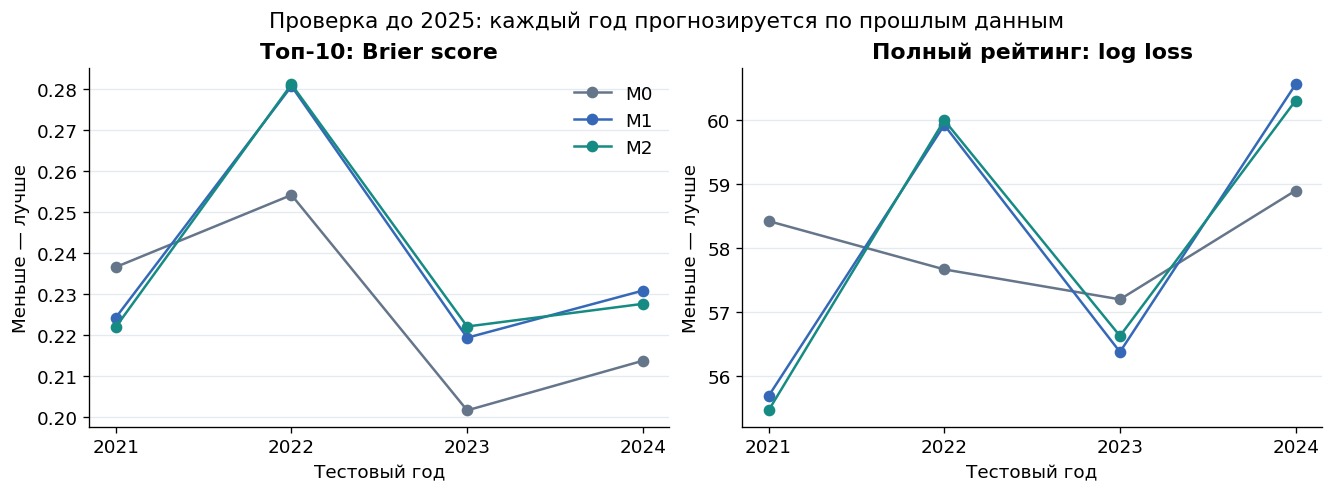
\includegraphics[width=.9\linewidth]{figures/A_core_annual_notebook.png}\\[4pt]
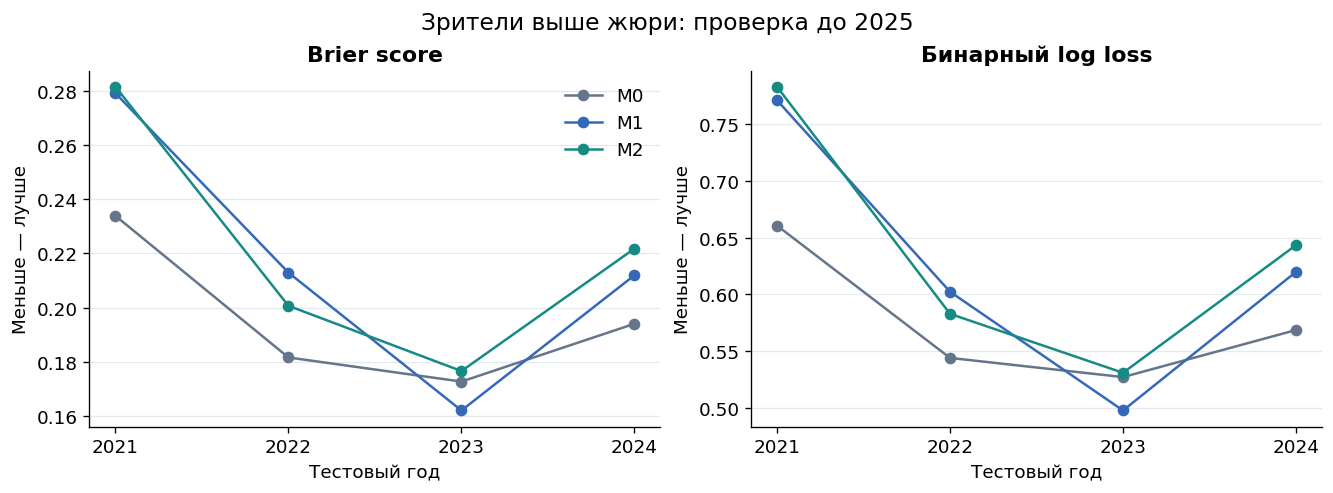
\includegraphics[width=.9\linewidth]{figures/B_core_annual_notebook.png}\\[4pt]
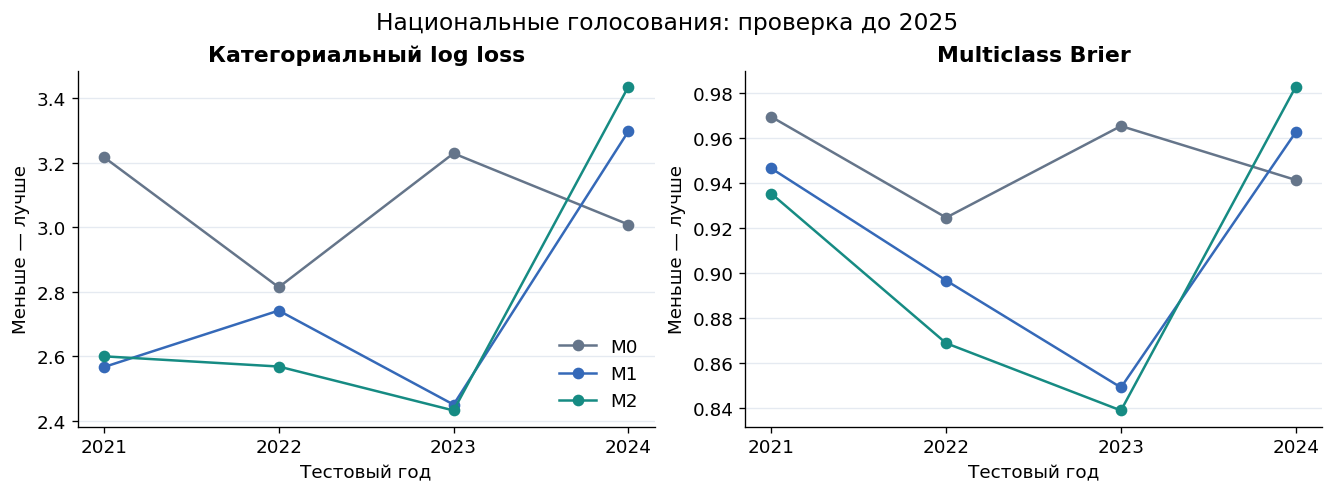
\includegraphics[width=.9\linewidth]{figures/C_core_annual_notebook.png}
\caption{Original no-odds evaluation plots from the supplied notebooks (A cell 17; B/C cell 15). Top row: A Brier and full-ranking log loss. Middle row: B Brier and binary log loss. Bottom row: C categorical log loss and multiclass Brier. All horizontal axes show test years 2021--2024; lower is better. Russian labels are retained from the original outputs. No plotted values were digitized or treated as exact numerical exports.}\label{fig:coreannual}
\end{figure}

\section{Bilateral support relative to other voters}\label{app:pairs}
For each eligible voter--recipient pair in a year, we subtract the proportion of the \emph{other} eligible voters who selected that recipient from the pair's own zero--one outcome. Averaging this difference over the years when the pair was eligible gives the colour in Figure~\ref{fig:regional}. This adjusts the descriptive comparison for the recipient's contemporaneous popularity, but not for every source of confounding.

\begin{figure}[H]\centering
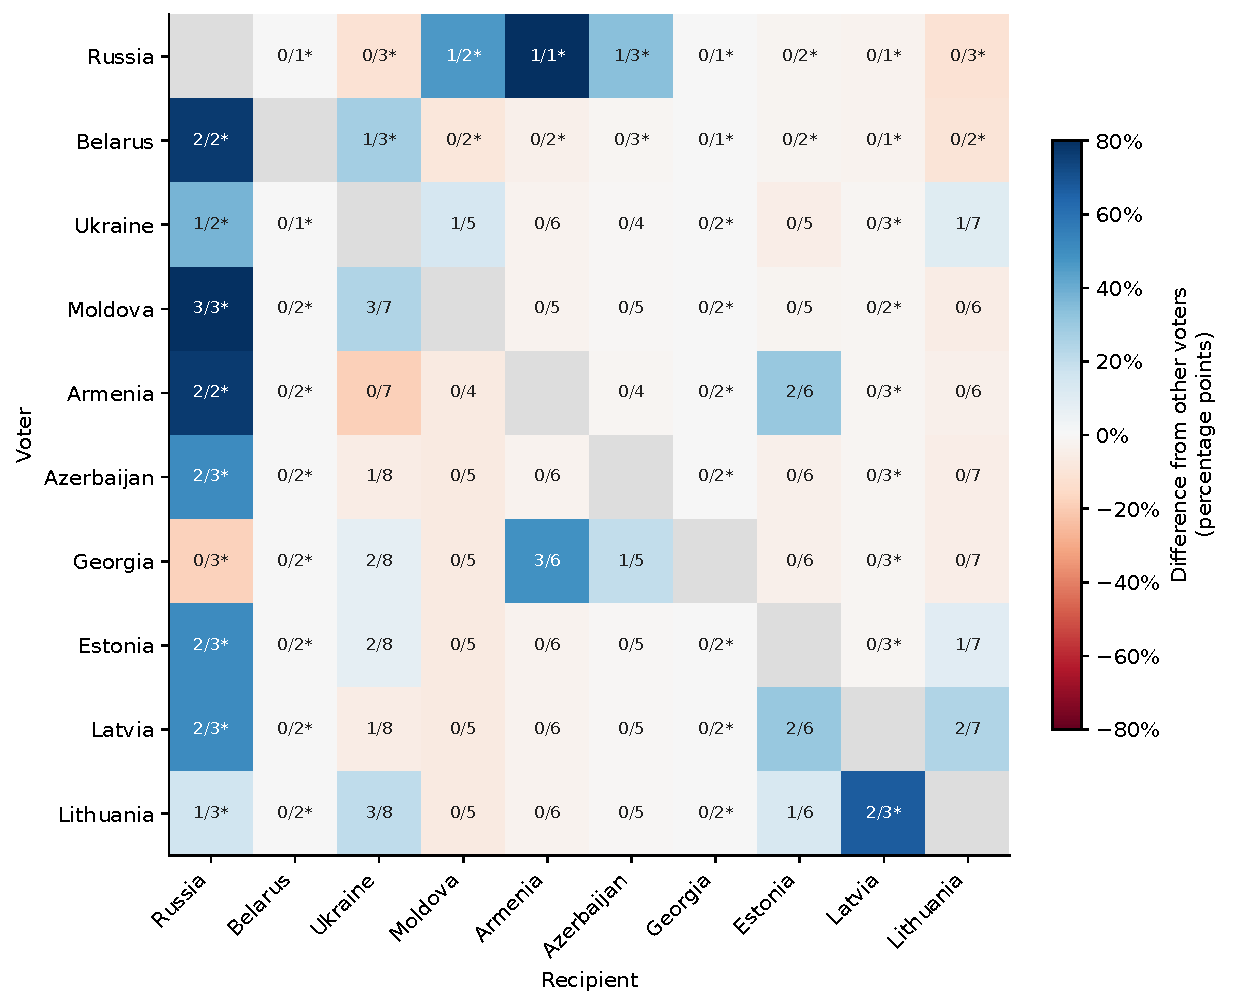
\includegraphics[width=.92\linewidth]{figures/regional_pairs.pdf}
\caption{Directed national first-place support in the ten-country regional subset specified in the descriptive notebook, 2016--2025. Labels are wins/eligible years; an asterisk marks fewer than four observations. Grey cells have no eligible observations. Colours show differences from other voters in percentage points. The notebook's additional countries selected for unusually strong observed links are omitted here, leaving the fixed regional subset. The comparison describes voting associations and cannot identify political or cultural causes.}\label{fig:regional}
\end{figure}
The unequal denominators matter: a pair with two eligible years can show a large difference with little information. Directed effects and shrinkage in C allow the model to represent persistent preferences while accounting for short histories. This figure uses same-year outcomes for description only; the model's past-pair-support predictor uses strictly earlier years.

\section{From proposal to implemented experiment}\label{app:proposal}
The proposal's three targets were retained. It envisaged overall results for 2004--2026, separate audience/jury ranks from 2009, and national televotes from 2014. The assembled coverage is 2008--2025 for A and 2016--2025 for B/C; matched A comparisons start in 2015 because of market coverage. No 2026 forecast is reported.

The proposal suggested Beta--Bernoulli baselines and probit extensions across the tasks. That specification was retained for B. A instead uses a Plackett--Luce ranking model, and C a categorical model, so their simulated or categorical forecasts respect the number of available winning positions. Their baselines learn historical recipient strength under the same likelihoods as the extensions. C uses directed pair effects; a voter-only intercept would cancel in its softmax likelihood. The matched no-odds runs were added after the lecturer's feedback on the presentation.

\section{Reproducibility and numerical provenance}\label{app:provenance}
\enlargethispage{3\baselineskip}
Market results come from the three \texttt{forecast\_*\_validation/market/} directories. No-odds aggregates are extracted from the supplied \texttt{matched\_core} notebooks, including the completed C notebook, and retain their four-decimal display precision. The models were not refitted for this report.

\begin{table}[H]\centering\small
\caption{Report evidence map. Notebook cell indices are zero-based.}\label{tab:map}
\begin{tabularx}{\linewidth}{lY}
\toprule
Item & Source\\\midrule
Tables \ref{tab:A}, \ref{tab:B}, \ref{tab:C} & Market: \texttt{development\_summary.csv}, \texttt{metrics\_2025.csv}. No odds: A cells 16/21; B and C cells 14/19.\\
Tables \ref{tab:Aranking}, \ref{tab:Caccuracy}, \ref{tab:increment}; Figure \ref{fig:increment} & Calculated from the same development/2025 summaries.\\
Figure \ref{fig:annual} & Market \texttt{development\_metrics\_by\_year.csv}.\\
Figures \ref{fig:songdata}--\ref{fig:geodata}, \ref{fig:regional}; Tables \ref{tab:annualdata}--\ref{tab:marketraw} & Descriptive notebook cells 3--9 and processed A/B/C tables.\\
Figures \ref{fig:ABforecast}--\ref{fig:Cforecast} & Market \texttt{comparison\_2025.csv}; no-odds HTML tables, A cell 21 and B/C cell 19.\\
Figures \ref{fig:calibration}, \ref{fig:nationalcounts} & Market calibration bins, 2025 probabilities and national outcomes.\\
Figure \ref{fig:coreannual} & Original embedded notebook PNGs; no numerical reconstruction.\\
Figure \ref{fig:effects} & C market \texttt{feature\_effects\_2025.csv}; posterior fitted through 2024.\\
Table \ref{tab:paired} & C market \texttt{paired\_comparisons.csv}; C no-odds cell 15.\\
Diagnostics & Market \texttt{verification.json}; no-odds A cell 25, B cell 23, C cell 25.\\
Table \ref{tab:prior} & No-odds A cell 19, B/C cell 17; market sensitivity CSVs retained.\\\bottomrule
\end{tabularx}
\end{table}

The accompanying \texttt{evidence/} directory contains numerical source tables and provenance records with source hashes. \texttt{build\_report\_assets.py} and \texttt{build\_extended\_assets.py} regenerate the LaTeX tables and vector figures from those CSVs. The no-odds annual plots are included as the original notebook PNGs; all figure files are in \texttt{figures/}. Forecast-level no-odds probabilities in the displayed notebook tables are rounded to 0.1 percentage point, while aggregate losses have four decimal places. Score comparisons use the saved aggregate losses; the rounded forecast tables are used only for the forecast-level figures.

The saved data-build verification records 21 matching final CSVs, matching values across six Excel sheets, and 46 passing tests; its JSON record is included in \texttt{evidence/}. The data, modelling notebooks, validation results, and reproduction instructions are available at \url{https://github.com/ivantanaevv/eurovision-forecasting}. In the repository, the report assets and evidence are stored under \texttt{report/}.

\begingroup
\small
\setlength{\bibsep}{3pt}
\begin{thebibliography}{9}
\bibitem[Blangiardo and Baio(2014)]{blangiardo2014}
Blangiardo, M. and Baio, G. (2014). Evidence of bias in the Eurovision song contest: Modelling the votes using Bayesian hierarchical models. \emph{Journal of Applied Statistics}, 41(10), 2312--2322. Open manuscript: \url{https://arxiv.org/abs/1308.6312}.
\bibitem[Adamska and Reiss(2025)]{adamska2025}
Adamska, K. and Reiss, J. (2025). Predicting Eurovision Song Contest Results: A Hit Song Science Approach. \emph{Transactions of the International Society for Music Information Retrieval}, 8(1), 93--107. \url{https://doi.org/10.5334/tismir.214}. Dataset: \url{https://github.com/kasiadamska/eurovision-song-science}.
\bibitem[EurovisionAPI(n.d.)]{api}
EurovisionAPI. Historical results and contestant data. \url{https://github.com/EurovisionAPI/dataset}. Frozen source revisions and checksums are recorded in the project data manifests.
\bibitem[Eurovision(n.d.)]{ebu}
Eurovision Song Contest. Official results archive and contest publications. \url{https://www.eurovision.com/}.
\bibitem[Eurovisionworld(n.d.)]{odds}
Eurovisionworld. Archived overall-winner odds, 2015--2025 excluding 2020. \url{https://eurovisionworld.com/odds/}. Historical pages follow \texttt{/odds/eurovision-YYYY}; price measurement timestamps are unverified.
\bibitem[Natural Earth(n.d.)]{ne}
Natural Earth. Populated places and administrative boundary data, v5.1.2, 1:10m. \url{https://www.naturalearthdata.com/downloads/10m-cultural-vectors/}.
\end{thebibliography}
\endgroup
\end{document}
